\subsection{Experimental Setup}
We evaluate our 2 learning method in a simulation environment on an overhand knot-tying task.
We use floating gripper with joint constraints to study the effects of trajectory transfer
without the complications of altering derived trajectories to incorporate joint constraints.

\subsubsection{Demonstrations}
The demonstrations we use to initialize the trajectory library are those used by
Schulman et al.~\cite{Schulmanetal_ISRR2013} for their experiments. The demonstrations
split the task of tying an overhand knot into 3 steps. Demonstrations were collected
by physically guiding a Willow Garage PR2 through these steps and opening or closing 
the grippers at the appropriate points. There are 36 demonstrations of full knot ties
in the data set in addition to several demonstrations that correct for common failures.
Point clouds were collected with a Kinect RGBD camera and filtered by color to extract
rope points. 

\begin{figure}
  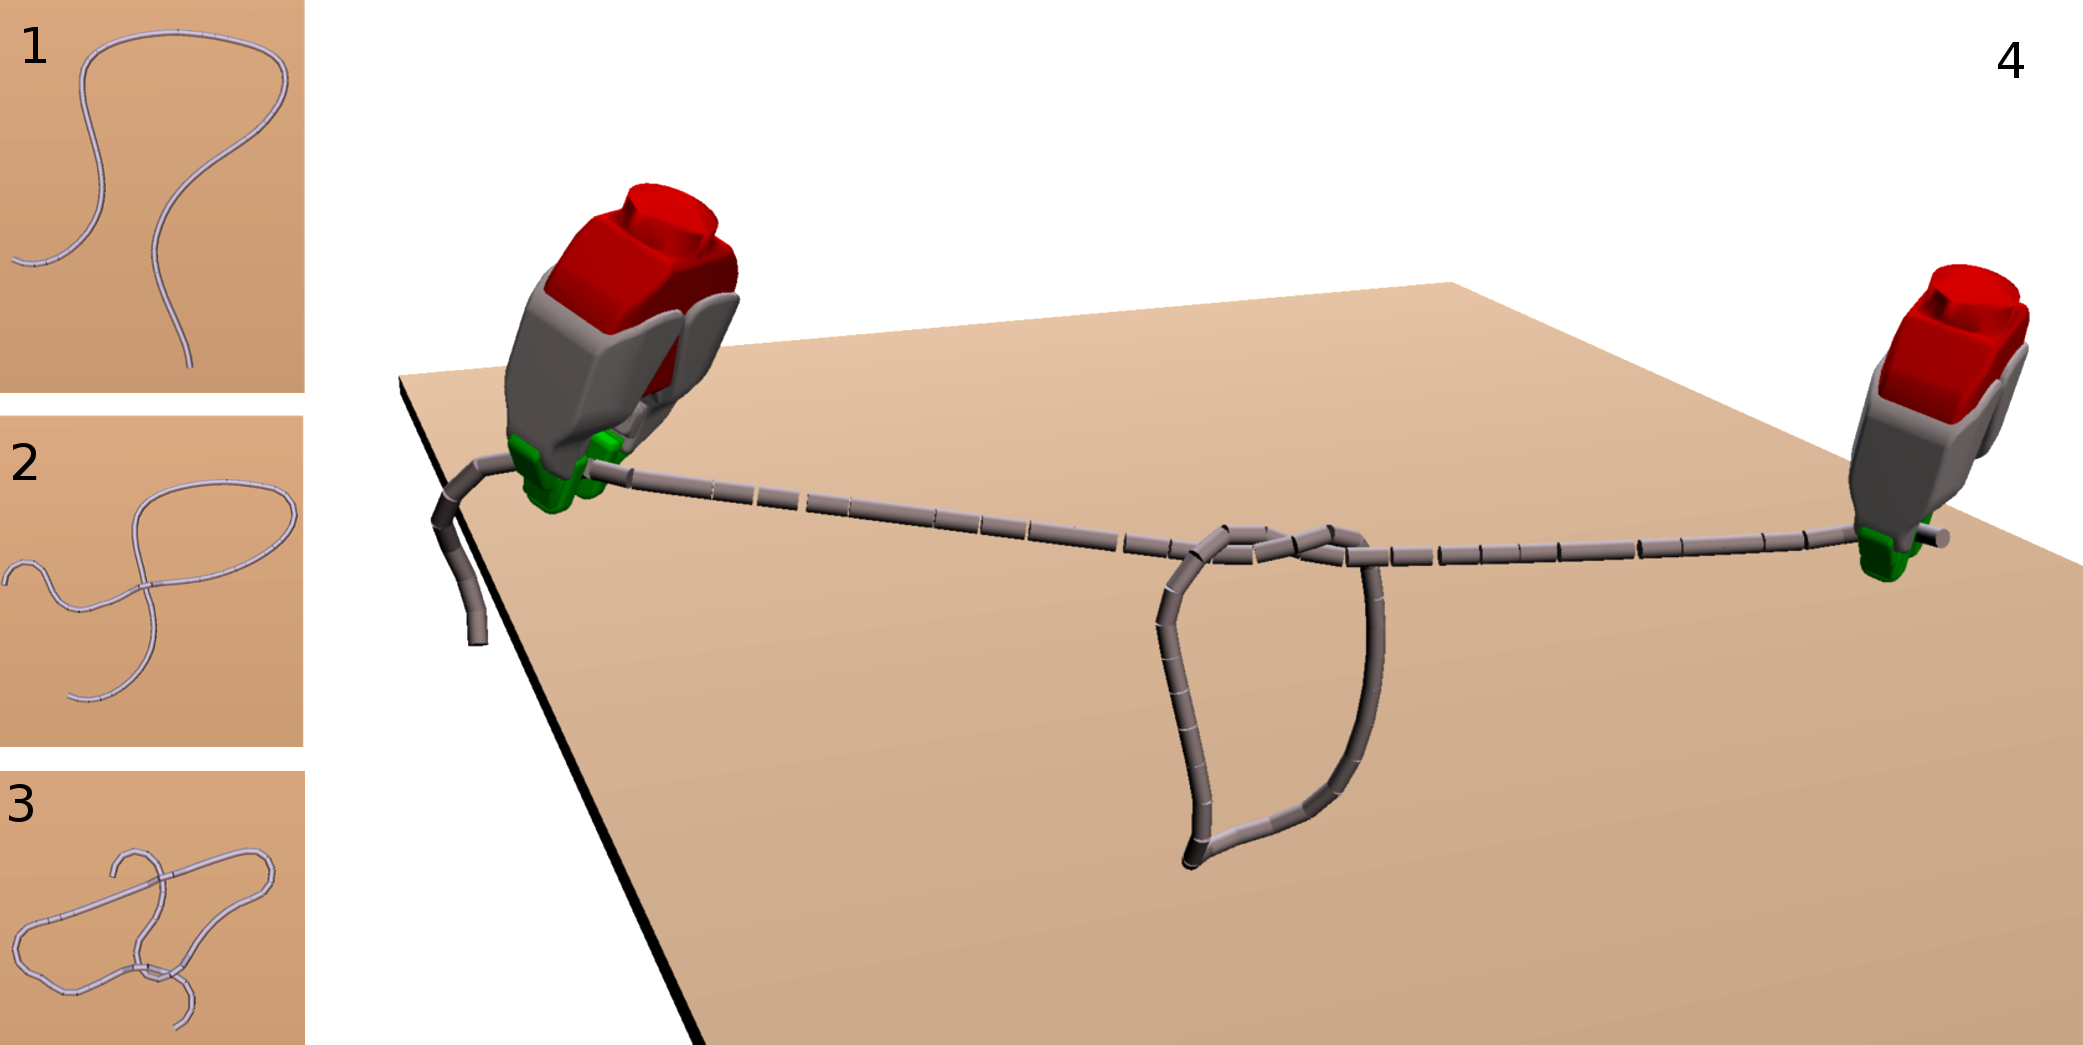
\includegraphics[width=\linewidth]{figs/cov.png}
  \caption{Example of the steps involved in an overhand knot-tying task in our simulated
           environment. The strandard demonstrations in our trajectory tie a knot as a 
           sequence of 3 steps.}
  \label{fig:knot_steps}
\end{figure}


\subsubsection{Simulation Environment and Task Distribution} 
The tasks we consider are simulations of an overhand knot tying tasks. 
We simulate a rope as a chain of cylinders linked by bending and torsional constraints.
Simulation is done through the use of Bullet Physics engine~\cite{Bullet_Physics}.

Our distribution over initial states is defined procedurally. We begin by uniformly
selecting an initial state from the demonstration. Then 7 points along the rope are 
drawn and subjected to 10cm of perturbation in a random direction. Finally a random
rotation between 0 and $\frac{pi}{4}$ is applied to the perturbed rope. We ran our
bootstrapping algorithms on initial states from this distribution and tested on a 
separate evaluation set.

\subsubsection{Training and Evaluation}
In order to explore the improvements from better modeling and compare with improvements
that come from better transfer of a particular trajectory, we ran two sets of experiments.
We generated 10 sequences of 170 states drawn IID from our initial state distribution.
We built a modified trajectory library for both approaches on each of the training sequences.
Training was accomplished by an initial exploration phase of 50 attempts where only the initial
demonstrations were used. Then there were 120 knot-tying attempts that chose and transferred
trajectories using the new techniques. We evaluated our bootstrapped libraries on an evaluation
set that consisted of 300 initial states that were held out from training.
